% CRITERIA	(2-3 pages)
	% -Check that each claim in the intro is addressed
	% -Forward reference evidence from a claim
	% -Present the experiments
	% -Analyze raw data
	
% OUTLINE
	% - Setup
		% - Criteria (Fitness)
			% - Distance (low weight since it doesn't really matter)
			% - Obstacle avoidance (Hight weight, mission critical)
			% - Minimize jerk (Mid weight)
		
		% - Touch breifly on encoding
			% - High order polynomial
			% - Chromozome - integer encoding
		% - Reporduction
			% - Random crossovers
		% - Mutation
			% - Defaults or Gusen's?
			% - Which worked out, why didn't the other?
		% - Initialization
			% - Random, pop size
		% - Termination
			% - Diversity convergence
			% - Or top half not coliding.
			% - Which worked out, why didn't the other?
			
		
	% - run with randomly generated environments (or at least 
		% - 1-5 objects
		% - placed randomly w/o overlap
		% - varying but constrained size
		% - fized start/end points
		% - Run 1000 times
		% - analyze data
		% - store data (map and the resultant path)

The Genetic Algorithm (GA) formed the basis for the experiemnts. Significant effort was expended setting up the GA in advance of testing, since without a well structured algorithm, the testing was sure to show poor results. The GA was implemented on Matlab, using the built-in GA libraries in order to avoid unnecessary development. While the base functionality was used, there remained many design considerations.

\subsection{Criteria and Fitness}
The aim of the implementation was to produce a path which minimized the obstacle collisions, length and jerk of the path represented by a polynomial function. The fitness of an individual was based on an equation considering these three criteria.

To consider obstacle collisions, the path was iterated along, and at each point along the path, a check was made to see if it was inside an obstacle. The number of units within an obstacle was penalized accordingly. Collisions resulted in high punishments to the fitness value of an individual. It was important to move the path around a collision point, for a single collision in the final solution will render that path invalid.

Length was calculated based on the integral line length formula. The weight of the line length was set to a medium penalty. This was due to the logic that it is more important to find a valid solution that collides with no obstacles than finding the shortest path between the two points.

Finally, the maximum jerk value of the line was found by iterating the length of the fourth derivative of the line and recording the maximum value of this derivative. The jerk weight was set to make reduction in the jerk as important as reduction in the path length.

\subsection{Configuration Space}
Commanding a robotic manipulator's position is complicated by the fact that it cannot be specified is X-Y-Z coordinates, but rather must be commanded using joint angles. Not only is this not intuitive for a human, but existing planning techniques function using more standard X-Y or X-Y-Z coordinate systems. As such, the robot's workspace was converted into a Configuration Space. Figure \ref{fig:ws2cs} shows both the workspace and the configuration space for a 2-DOF robot in an arbitrary workspace. The robotic manipulator's two degrees of freedom are denoted by the blue and red lines (each DOF respectively). The alloable robot configurations denoted in the Configuration Space by whitespace, while collisions are denoted by black.

\begin{figure}[h]
	\centering
	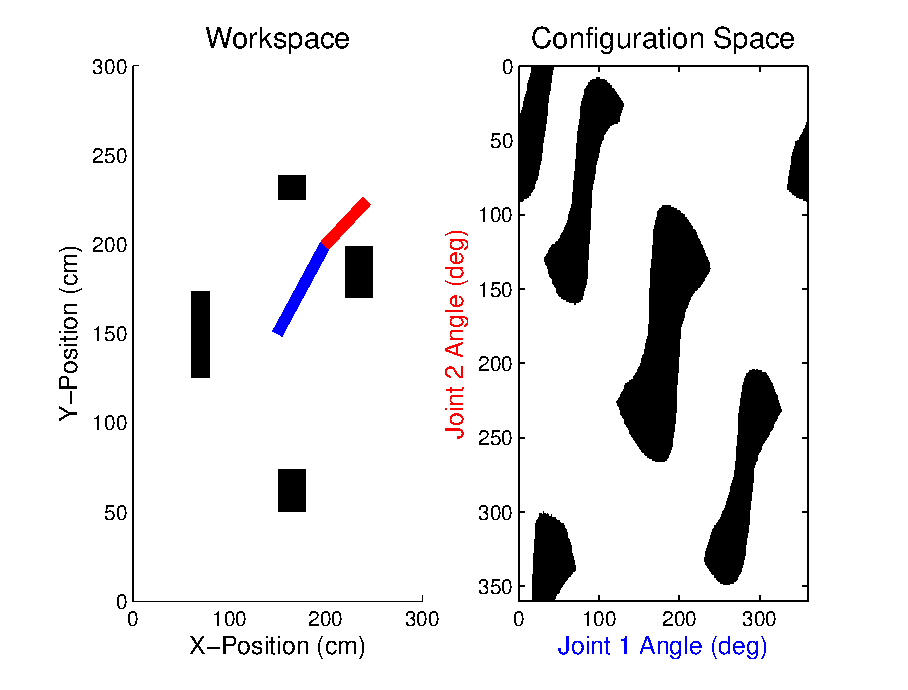
\includegraphics{./figures/wp2cs.eps}
	\caption{Conversion from robot workspace to configuration space }
	\label{fig:ws2cs}
\end{figure}

In the configuration space, robot tracjectories can be easily identified by either a human or a motion planning algorithm. This angle-angle plot can then be used to implement a polynomial trajectory, of which optimal coefficients can easily be solved using a Genetic Algorithm. The parameterized trajectory is denoted in Equation \ref{eq:polyTraj}.

\subsection{Population Initiatlization}
The population was randomly initialized with coefficient values in the range of \-100 to 100. This range was imposed on the coefficients as it was found to provide a good compromise between promoting function manipulation while at the same time keeping it under control so that changes to coefficients did not make too drastic a change to the shape of the path.

The population size was chosen to be 75. This population number was found to provide the necissary diversity in the population. Lower population values were found to converge to non-ideal solutions.

\subsection{Encoding}
The GA was developed using a linear encoding scheme, where a chromosome was defined to be an array of the polynomial function's coefficients (denoted as $\{P_0, \ldots, P_3\}$ in Equation \ref{eq:polyTraj}). Therefore, the GA would ultimately return the ideal set of coefficients for a function which would describe the optimal path for the robotic manipulator. These coefficients were limited to a range of [-500,500], since larger coefficients guarantee an invalid path since it would be too large and leave the workspace. While larger coefficients do not adversely affect the result of the algorithm, the increased diversity requires significantly larger computational resources which were not avaliable.

\subsection{Linear Constraints}
The path planning problem is a challenging optimization problem due to the various constraints
involved. The goal is to generate a path that avoids all obstacles, as well as minimize the path length and
minimize jerk. The problem is further constrained by the start and end points. The generated polynomial path must go through these desired start and end points.

To solve this constrained optimization problem, linear equality constraints are used. Linear equalities
have the form :

\begin{equation}
A_{eq}x = b_{eq}
\end{equation}

where x are the variables being optimized. For this project, the optimization variables are the
coefficients of the polynomial.

For example, a second order polynomial $y = A + Bx + Cx^2$ through points $[1 2]$ and $[10 5]$ would have linear constraints of the form:
\begin{equation} 
\begin{bmatrix}
1 & 10 & 10^2 \\
1 & 5 & 5^2
\end{bmatrix}
\begin{bmatrix}
A \\
B \\
C \\
\end{bmatrix} = 
\begin{bmatrix}
10 \\
5 \\
\end{bmatrix}
\end{equation}
\subsection{Selection}
A tournament selection method was used in this implementation. 2 individuals were chosen for each tournament. This allowed for an acceptable tradeoff between choosing a fit parent while promoting diversity in the offspring. This was one approach used to increase the diversity of the population when it was observed that the algorithm was getting stuck in local minima.

\subsection{Reproduction and Mutation}
A heuristic reproduction method was used wherein the child is generated by taking the mean of the coefficients of the two parents, and then biased to resemble the parent. In our implementation, the child was biased 20\% towards the most fit parent using formula \ref{crossoverEq}.

\begin{equation} \label{crossoverEq}
child_i = parent_{i2} + 1.2 * (parent_{i1} + parent_{i2})
\end{equation}

As is common in non-binary encoded GA problems, the crossover method used in this implementation is based on a mean of the parents' genes. This is a key distinction from a traditional point crossover method, as it allows the genes to evolve from values that were not present in the initial population. If point crossover methods had been used, the best case scenario would involve the optimal configuration of coefficients from the initial, random population.

Mutation was achieved applyinh a completely random mutation to a coefficient within the inidvidual selected to be mutated. In order to satisfy the linear constraints of the start and end points, if the function was rendered invalid by the mutation, a new random coefficient was chosen instead.

\subsection{Termination}
The termination criteria allow the GA to determine when it has reached the optimal solution to the problem. In this implementation, a termination criteria based on convergence of the fitness function was used. The mean fitness value over ten generations was averaged. When the this averaged mean fitness value converged within 0.001 units, the algorithm was terminated. This is representative of a situation where the diversity of the function has been reduced, and the algorithm has converged on a minimum fitness value.

\subsection{Experiment} \label{sec:experiment}
In order to assess the performance of the GA approach, an extensive experiment was devised. The algorithm was run 600 times on 15 sets of randomly generated points in 3 environments with randomly positionned obstacles. Invalid combinations of point sets were removed from the dataset and new points were randomly generated to replace them. The environments were chosen to represent environments which were sparsely populated with obstacles, through to dense population with obstacles. The results obtained by this experiment are presented in the following section.